 \documentclass[3p]{elsarticle}
%\documentclass[preprint]{elsarticle}

% The preceding line only needs to identify funding in the first footnote. If that is unnecessary, please comment on it.

% =====================  Clean & Stable Preamble (single-column)  =====================

\usepackage{amsmath, amsfonts, amsthm, bm}
\usepackage{amssymb}

\theoremstyle{remark}
\newtheorem*{remark}{Remark}

\usepackage{graphicx}
\usepackage{svg}         

\usepackage{array}         
\usepackage{booktabs}      % \toprule \midrule \bottomrule
\usepackage{multirow}
\usepackage{threeparttable}

\usepackage{stfloats}

\usepackage{algorithm}
\usepackage{algorithmic}   

\usepackage[T1]{fontenc}
\usepackage{textcomp}
\usepackage{pifont}      
\usepackage{enumitem}

\usepackage{url}
\usepackage{pdfpages}
\usepackage{verbatim}
\usepackage{subcaption}    
\usepackage{multicol}
\usepackage{xcolor}        
\usepackage{soul}          
\usepackage{tcolorbox}

\usepackage{tabularx}           
\newcolumntype{Y}{>{\raggedright\arraybackslash}X}   
\newcolumntype{C}{>{\centering\arraybackslash}X}     

% ===========================
% ===========================
\newtheorem{theorem}{Theorem}
\newtheorem{definition}{Definition}
\newtheorem{lemma}{Lemma}
\newtheorem{corollary}{Corollary}
\newtheorem{assumption}{Assumption}

% ===========================
% ===========================
\usepackage{tikz}
\newcommand*\emptycirc[1][1ex]{\tikz\draw (0,0) circle (#1);}
\newcommand*\halfcirc[1][1ex]{%
  \begin{tikzpicture}
    \draw[fill] (0,0)-- (90:#1) arc (90:270:#1) -- cycle ;
    \draw (0,0) circle (#1);
  \end{tikzpicture}}
\newcommand*\fullcirc[1][1ex]{\tikz\fill (0,0) circle (#1);}

\newcommand{\sharesig}{\mathsf{ShareSig}}
\newcommand{\ta}{\mathsf{TA}}
\newcommand{\txr}{\mathsf{TX}_r^I}
\newcommand{\blockr}{\mathsf{B}_r^I}
\newcommand{\blockrr}{\mathsf{B}_{r-1}^I}
\newcommand{\blockrrr}{\mathsf{B}_{r-2}^I}
\newcommand{\mprop}{m_\text{prop}}
\newcommand{\propose}{\mathtt{PROPOSE}}
\newcommand{\sigmaI}{{\sigma_I}}
\newcommand{\mpre}{m_\text{pre}}
\newcommand{\prepare}{\mathtt{PREPARE}}
\newcommand{\sigmai}{{\sigma_i}}
\newcommand{\recon}{\mathsf{Reconstruct}}
\newcommand{\Sigmapre}{\Sigma_\text{pre}}
\newcommand{\prepared}{\mathbf{prepared}}
\newcommand{\mcom}{m_\text{com}}
\newcommand{\commit}{\mathtt{COMMIT}}
\newcommand{\committed}{\mathbf{committed}}
\newcommand{\vote}{\mathtt{VOTE}}
\newcommand{\Sigmacom}{\Sigma_\text{com}}
\newcommand{\mvote}{m_\text{vote}}
\newcommand{\Sigmarr}{\Sigma_{r-1}}
\newcommand{\Sigmar}{\Sigma_{r}}
\newcommand{\inl}{{I\in[n_L]}}
\newcommand{\blockrnl}{\mathsf{B}_r^{n_L}}
\newcommand{\bft}{\mathsf{BFT}}
\newcommand{\bblockr}{\overline{\mathsf{B}}_r^I}
\newcommand{\DRG}{\mathsf{DRG}}
\newcommand{\setup}{\mathsf{Setup}}
\newcommand{\kzg}{\mathsf{KZG}}
\newcommand{\nizk}{\mathsf{NIZK}}
\newcommand{\nizkvf}{\mathsf{NIZK.Vf}}
\newcommand{\zksnark}{\mathsf{zkSNARK}}
\newcommand{\bg}{\mathbb{G}}
\newcommand{\ff}{\mathbb{F}}
\newcommand{\keygen}{\mathsf{KeyGen}}
\newcommand{\kzgcommit}{\mathsf{Commit}}
\newcommand{\decrypt}{\mathsf{Decrypt}}
\newcommand{\hash}{\mathsf{H}}
\newcommand{\vrf}{\mathsf{VRF}}
\newcommand{\ser}{\mathsf{Ser}}
\newcommand{\cmark}{\ding{51}} 
\newcommand{\xmark}{\ding{55}} 

\definecolor{mygray}{gray}{0.6}
\definecolor{myyellow}{rgb}{0.9, 0.7, 0.0}
\definecolor{mygreen}{rgb}{0.0, 0.5, 0.0}
\definecolor{mypurple}{rgb}{0.75, 0.0, 0.75}

\newcolumntype{Y}[1]{>{\centering\arraybackslash}p{#1}}

% ===========================
% ===========================
\journal{Computers and Electrical Engineering}
% ========================================================================
\usepackage{CJKutf8}

\biboptions{sort&compress}

\begin{document}



\begin{frontmatter}
\title{
CleVer: A Compute-and-Leave Anonymous Verification Framework for General Purpose Computation
}

% ---------- Authors ----------
\author[bh]{Qiyuan Gao\corref{cor1}}
\ead{gaoqy@buaa.edu.cn}

\author[bh]{Qianhong Wu}
\ead{qianhong.wu@buaa.edu.cn}

\author[bh]{Qi Liu}
\ead{liuqi2032472260@163.com}

\author[bh]{Junxiang Nong}
\ead{fpdqwq@yeah.net}

% ---------- Corresponding author ----------
\cortext[cor1]{Corresponding author.}

% ---------- Affiliation ----------
\address[bh]{Beihang University, Beijing, China}
\begin{abstract}
Verifiable computation is essential for ensuring correctness in decentralized systems, yet existing ap- proaches rely heavily on circuit-based proofs, task decomposition, or trusted hardware, which introduce high overhead and limit generality. To address these challenges, we propose CleVer, a compute-and-leave anonymous verification framework for general-purpose computation. 

CleVer avoids circuit-based proof generation by using snapshot-based state transitions, enabling single-step dispute resolution without task decomposition. We design a cumulative staking incentive mechanism that guarantees profitability for honest verifiers and enforces bounded finality under adversarial budgets. Furthermore, we introduce an anonymous verifier protocol to prevent targeted attacks and collusion. Security is analyzed under a formal threat model, and experiments demonstrate that CleVer significantly reduces verification rounds and on-chain burden compared with existing optimistic-verification frameworks. Our results show that CleVer provides an efficient, incentive-aligned, and privacy-preserving foundation for scalable off-chain computation.
\end{abstract}

\end{frontmatter}




\section{Introduction}

In the rapidly developing field of distributed computing, the integrity and reliability of remotely executed computations are becoming increasingly significant~\cite{surveyofcloud, CEE-security}. Verifiable computation, as a key technology, enables clients to verify the correctness of computation results obtained from untrusted servers without having to repeat the computation themselves~\cite{blkvc-review,vc-survey,v3rified}. This technology not only enhances the security of cloud computing environments, but also supports new applications in the field of outsourced computing. Although verifiable computation has broad potential and prospects, it is still quite challenging to verify large-scale general computations based on current mature solutions.

Existing approaches to verifiable computation are dominated by cryptographic and mathematical methods, where computation tasks are transformed into circuits and proofs are generated for efficient verification~\cite{NOVA, Orion, transparentZK}. Although effective for small-scale tasks, circuit generation becomes prohibitively expensive for large or complex computations, and the requirement to rewrite tasks with specific toolchains limits general-purpose applicability. Blockchain systems~\cite{CEE-blockchain, CEE-blockchain-verify} further highlight these challenges: while consensus ensures correctness of smart contract execution~\cite{wood2014ethereum, taherdoost2023smart, CEE-blockchain-consensus, oliva2020exploratory}, it requires all nodes to redundantly execute contracts, leading to substantial overhead~\cite{consensussurvey, wang2019survey}, and cannot support computations beyond block capacity. These limitations motivate a deeper examination of the challenges in current verifiable computation frameworks.


\subsection{Background and Problem Statement}

This section elaborates on the challenges identified above.

\textbf{Cryptographic approaches face efficiency bottlenecks.}  
Most existing solutions to verifiable computation rely on cryptographic reductions, such as zero-knowledge proofs (ZKP) or succinct non-interactive proofs of knowledge. In these schemes, computation tasks are logically decomposed into circuits, and proofs are generated to allow verifiers to check results without re-execution. While these techniques enable succinct verification, the costs of circuit generation and proof construction grow prohibitively large for complex workloads. Furthermore, the requirement to rewrite tasks using specific toolchains limits the applicability to arbitrary general-purpose computations.

\textbf{Consensus excludes complex computations.}  
Blockchain systems provide a representative environment in which verifiable computation is indispensable. Consensus ensures deterministic finality and correctness of executed tasks, but requires consensus nodes to redundantly execute them, incurring heavy computational overhead. Moreover, consensus protocols are inherently designed for fast agreement rather than for verifying long and complex computation paths. As a result, on-chain verification cannot feasibly support general-purpose computation beyond block size or gas capacity constraints.

\textbf{Verification suffers from weak finality and incentives.}  
To overcome on-chain limitations, many frameworks shift computation off-chain and rely on on-chain consensus only for arbitration in case of disputes. While this improves scalability, it introduces weaker finality, coordination complexity, and dependence on assumptions such as trusted hardware. More critically, most systems lack mechanisms to properly align incentives with verifier effort. Rational verifiers may adopt \textit{lazy verification} strategies---skipping actual validation to minimize costs while still claiming rewards---leading to the \textbf{Verifier Dilemma}~\cite{luu} and undermining overall system integrity. Furthermore, the public nature of verifier identities exposes them to bribery, collusion, and denial-of-service attacks, compromising independence and eroding the trust foundation of the verification process.


\subsection{The Compute-and-Leave Protocol}

To address the limitations of current verification frameworks, we introduce \textbf{CleVer}, a Compute-and-Leave model tailored for general-purpose computation. CleVer leverages a snapshot-based optimistic verification strategy with single-step challenge resolution, enabling high-efficiency validation while maintaining strong security and economic robustness.

\textbf{Snapshot-Based Verification.}  
CleVer models general computation as a finite state machine, with the execution trace captured through a series of intermediate state snapshots. These snapshots are triggered when the accumulated instruction weight exceeds a fixed threshold, ensuring each snapshot interval aligns with on-chain block processing constraints. This design eliminates the need for full-task re-execution or circuit compilation, enabling efficient single-step dispute resolution.

\textbf{Cumulative Challenge Incentives.}  
To prevent denial-of-service attacks on the challenge interface, CleVer introduces a cumulative staking incentive mechanism. The stake from each rejected malicious challenge is carried forward to reward subsequent challengers, with the cumulative reward defined by a monotonically increasing function $f(s)$ over the round index $s$. This design allows flexibility in choosing different forms of $f(s)$—such as exponential, logarithmic, or polynomial growth—depending on system requirements. By ensuring that adversarial costs grow rapidly while honest challengers are economically motivated, CleVer reduces the number of rounds needed to reach finality and maintains fairness and efficiency in dispute resolution.

\textbf{Succinct Workload Proofs.}  
CleVer mitigates the Verifier Dilemma by requiring verifiers to submit succinct proofs of their verification effort. By comparing the instruction-weight trace between verifier and executor, the system can confirm whether sufficient verification was performed. This mechanism disincentivizes lazy behavior and aligns verifier rewards with actual effort, maintaining the integrity of the verification process.

\subsection{Our Contributions}

The key contributions of CleVer are summarized as follows:

1. We propose CleVer, a novel verifiable computation framework that supports general-purpose computation without requiring zero-knowledge proofs or trusted hardware, which can be deployed in blockchain and consensus-based environments.

2. CleVer introduces a state-snapshot-based single-step verification model, which enables efficient and parallelizable verification, achieving rapid finality even for complex workloads.

3. We design incentive-compatible mechanisms, combining verification workload proofs with a cumulative staking incentive scheme, which jointly mitigate the Verifier Dilemma and strongly deter malicious challenges.

4. To achieve verifier anonymity, CleVer implements an anonymous verifier staking and election protocol. In this protocol, the ZKP component functions solely as an auxiliary cryptographic tool for identity protection, while the computation verification mechanism and the ZKP component follow two distinct design paths. This design effectively reduces the risks of bribery and targeted attacks.

\subsection{Structure of this Paper}

The remainder of this paper is structured as follows: Section 2 provides an overview of related work. Section 3 introduces the necessary preliminaries. Section 4 describes the system model. Section 5 elaborates on the verification mechanism of CleVer, while Section 6 presents its anonymous verification approach. Section 7 conducts a security analysis of CleVer. Section 8 evaluates CleVer through experimental testing and compares it with existing projects. Finally, Section 9 concludes the paper.

\begin{table}[htbp]
  \centering
  \caption{Comparison of blockchain verification capacity expansion projects}
  \label{tab:Comparison}

  \begingroup
  \setlength{\tabcolsep}{5pt}
  \renewcommand{\arraystretch}{1.2}
  \normalsize

  \resizebox{\linewidth}{!}{%
  \begin{tabular}{
      l
      p{0.30\linewidth}
      c c c c
  }
    \toprule
    \textbf{Protocol} &
    \textbf{Security Assumption} &
    \textbf{Incentive Compatibility} &
    \textbf{Solved Verifier Dilemma} &
    \textbf{Verifier Anonymity} &
    \textbf{Complex Comp.} \\
    \midrule

    \textbf{Sharding}~\cite{shardingsurvey} &
    Consensus threshold &
    \cmark & \cmark & \cmark & \xmark \\

    \textbf{State Channel}~\cite{GenSTATE} &
    Anyone\mbox{-}can\mbox{-}challenge trust &
    \xmark & \xmark & \xmark & Partial \\

    \textbf{Arbitrum}~\cite{ARBITRUM1} &
    Anyone\mbox{-}can\mbox{-}challenge trust &
    \xmark & \xmark & \xmark & Partial \\

    \textbf{Optimism Rollup}~\cite{opRollups} &
    Anyone\mbox{-}can\mbox{-}challenge trust &
    \xmark & \xmark & \xmark & Partial \\

    \textbf{ZK Rollup}~\cite{zksync_whitepaper,ethZkRollups} &
    Cryptographic circuit soundness &
    \xmark & \cmark & \xmark & Partial \\

    \textbf{TEE}~\cite{SGXICDE} &
    Trusted hardware &
    \xmark & \cmark & \xmark & \cmark \\

    \midrule
    \textbf{CleVer} &
    Anyone\mbox{-}can\mbox{-}challenge trust &
    \cmark & \cmark & \cmark & \cmark \\
    \bottomrule
  \end{tabular}%
  }
  \begin{tablenotes}
    \footnotesize
    \item This table compares representative blockchain verification capacity expansion schemes by security assumptions, incentive compatibility, ability to solve the Verifier Dilemma, verifier anonymity, and complex computation support. It highlights design trade-offs and shows that CleVer offers a balanced mix of security, incentives, privacy, and computational flexibility.
  \end{tablenotes}
  \endgroup
\end{table}

\section{Related Work}

Research on verifiable computation has mainly followed three technical paths: cryptographic proof systems, consensus-backed verification, and trusted hardware.

\subsection{Cryptographic Approaches}

Cryptographic methods such as Zeroknowledge Proofs(ZKP)\cite{NOVA,antman,zhang2021pipezk,transparentZK,Orion} transform computations into circuit-based proofs, allowing verifiers to check correctness without re-executing tasks. These approaches provide strong security guarantees and succinct verification, but they face high proof generation costs, significant communication overhead, and, in many cases, the requirement of trusted setup parameters. Such challenges limit their applicability to large-scale, general-purpose computations.

\subsection{Consensus and Blockchain Approaches}

Another path of research relies on consensus-based verification, where computation tasks confirmed beyond a security threshold are regarded as correct. Blockchain systems~\cite{wood2014ethereum} are a typical instantiation, in which multiple nodes redundantly execute tasks and confirm results through protocol agreement. While consensus ensures deterministic finality, it incurs heavy computational overhead, reduces throughput, and constrains computations within block boundaries. Recent advances such as parallel execution, sharding, and optimized consensus protocols~\cite{ICP,solana-doc,shardingsurvey} improve efficiency to some extent, but they do not remove the fundamental trade-offs between scalability, decentralization, and performance. Moreover, the execution model itself remains bound by block intervals, limiting its ability to handle computations beyond block capacity.
Table~\ref{tab:Comparison} compares these blockchain based verification schemes.

\subsection{Trusted Hardware Approaches}

Trusted execution environments (TEEs), such as Intel SGX or ARM TrustZone~\cite{SGX31,SGXICDE}, provide another approach by executing computations within secure enclaves. TEEs can offer high performance and confidentiality, but their correctness depends entirely on hardware integrity. Once compromised, they introduce a single point of failure, raising concerns about robustness and trust assumptions.

\textbf{In summary,} cryptographic approaches provide rigorous proofs but are costly and inflexible; consensus-based methods guarantee finality but suffer from redundancy and scalability constraints; and trusted hardware improves efficiency only at the expense of strong trust assumptions. None of these directions satisfies the need for efficient, incentive-compatible, and general-purpose verifiable computation, which motivates the design of CleVer.


\section{Preliminaries}


\subsection{WebAssembly}
WebAssembly (Wasm)~\cite{wasmempirical,wasmsok,wasmweb} is a portable, low-level bytecode format designed for safe and efficient execution across various platforms. Originally developed to enhance the performance of web applications, WebAssembly provides a compact and fast runtime environment that supports multiple programming languages, such as C, C++, and Rust, allowing them to run in a sandboxed environment. Its design emphasizes cross-platform compatibility, close-to-native performance, and security, making it an ideal choice for resource-constrained or performance-critical applications. In the context of blockchain, WebAssembly has been adopted as a virtual machine (VM) for executing smart contracts, offering advantages such as faster execution, reduced resource consumption, and support for diverse programming languages, thereby addressing some of the limitations of traditional virtual machines like the Ethereum Virtual Machine (EVM).

\subsection{Aztec Private Transfers.}
Aztec~\cite{aztec2021whitepaper} enables confidential asset transfers on Ethereum by representing each asset as a note: $N = \textsf{Commit}(v, \rho, pk)$, where \( v \) is the value, \( \rho \) is randomness, and \( pk \) is the recipient’s public key. A private transfer consumes input notes \( \{N_i\} \) and creates output notes \( \{N_j'\} \), preserving value: $\sum_i v_i = \sum_j v_j'$. A zero-knowledge proof \( \pi \) is generated to prove correctness and ownership without revealing \( v \), \( \rho \), or \( pk \). This construction guarantees value privacy, sender/receiver anonymity, and public verifiability.

\section{System Model}

The primary goal of CleVer is to enable fast and efficient verification of general complex computational tasks on the blockchain while addressing the limitations of previous related works.

In this section, we first introduce the workflow in CleVer and the roles of different participants. Then, we analyze the security threat model and present the design objectives of CleVer.


We formally define the components of our off-chain computational verification model as follows:

\begin{definition}[Computational Task]\label{def-task}
A computational task $\tau$ is defined as:
\[
\tau = \langle \sigma_{\text{start}}, \sigma_{\text{end}} \rangle
\]
where $\sigma_{\text{start}}$ and $\sigma_{\text{end}}$ represent the initial and final states of the task. Tasks whose complexity exceeds the processing capacity of on-chain consensus are executed off-chain and referred to as complex computations.
The execution of $\tau$ is modeled as a finite state machine:
\[
\sigma_{\text{start}} \to \sigma_1 \to \sigma_2 \to \cdots \to \sigma_{\text{end}}
\]
\end{definition}

Each state $\sigma_i$ encapsulates both the intermediate data and the executed code context required for progression.\footnote{That is, we assume $\sigma_i$ includes all necessary context, such as execution data and the corresponding code fragment. Therefore, we omit explicit representation of these elements in the transition rules for simplicity.}

\begin{definition}[Adjacent State Transition Rule]\label{def:snap-standard}
The state transition between adjacent computation states follows:
\[
\text{Com}(\sigma_i, T_w) \rightarrow \sigma_{i+1}
\]
The system executes the computation from state $\sigma_i$ until the accumulated instruction weight reaches a predefined threshold $T_w$. At this point, a new snapshot is recorded as $\sigma_{i+1}$, and the weight counter resets for the next segment.
\end{definition}

The threshold $T_w$ reflects the block time constraints on the underlying blockchain. We pre-measure instruction weights in the WASM-SNAP environment(A WasmEdge-based runtime environment we developed which can save a snapshot of the current runtime state based on the instruction weight) to ensure that each transition segment remains verifiable within a single block.

\begin{definition}[Verifier Set and Endorsements]\label{def:verifier-set}
Let $\mathcal{V} = \{V_1, V_2, \dots, V_n\}$ be the set of verifiers assigned to task $\tau$. Each $V_i \in \mathcal{V}$ operates independently and is responsible for reviewing the state transitions of $\tau$.
\end{definition}

In CleVer, each verifier is selected anonymously and operates independently under rational and non-colluding assumptions. During the verification window, a verifier may submit either an \textit{endorsement} (indicating correctness) or a \textit{challenge} (if any error is detected) to the on-chain contract.

\begin{definition}[Verification Rule]\label{def:verify-rule}
The correctness of $\tau$ is validated in two phases:
\begin{itemize}
    \item \textbf{Verifier Endorsement Phase:} All $V_i \in \mathcal{V}$ independently review $\tau$ and optionally issue endorsements.
    \item \textbf{Challenge Phase:} If any $V_i$ detects an error, it submits a challenge on-chain during the verification window.
\end{itemize}
If no valid challenge occurs within the window, the system deems $\tau$ correct. Irrelevant or malicious challenges are penalized through the staking mechanism.
\end{definition}

% \renewcommand{\arraystretch}{1.15}
\begin{table}[htbp]
    \centering
    \caption{Notations}
    \label{Notations}
    \footnotesize
    \begin{tabular}{>{\centering\arraybackslash}p{0.18\linewidth} >{\arraybackslash}p{0.7\linewidth}}
    \toprule
    \textbf{Notation} & \textbf{Description} \\
    \midrule
    $\tau$ & Computational task under verification. \\
    $\sigma_i$ & $i$-th intermediate state snapshot of $\tau$. \\
    $Ver(\cdot)$ & Basic verification operation. \\
    $\mathcal{V}, V_i$ & Verifier set $\mathcal{V}$ and verifier $V_i$. \\
    $f(s)$ & Staking function: deposit required in round $s$ (strictly increasing). \\
    $F(t)$ & Cumulative staking: $F(t)=\sum_{i=1}^{t} f(i)$, total deposits up to round $t$. \\
    $\mathrm{Pool}(s)$ & Reward pool before round $s$: $B+\sum_{i=1}^{s-1} N_i f(i)$, with $B$ the base bounty and $N_i$ invalid challengers in round $i$. \\
    $G, H$ & Generator points of the elliptic curve group. \\
    $\pi$ & NIZK proof for verification correctness. \\
    $C_i$ & Stake commitment of $V_i$. \\
    $r_i, v_i$ & Verifier’s random ID and stake value. \\
    $B, A, R$ & Node types: Byzantine, Altruistic, Rational. \\
    $W_\tau$ & Total number of executed instructions in task $\tau$, used to characterize workload size. \\
    $a_\tau$ & Cost of performing a single verification operation on task $\tau$. \\
    $\mathit{fee}$ & On-chain transaction or consensus fee required for finalizing a verification step. \\
    $B_{\mathcal{A}}$ & Adversary's available budget for launching blocking attacks or malicious challenges. \\

    \bottomrule
    \end{tabular}
\end{table}

\begin{definition}[Basic Verification Unit]\label{def:basic-unit}
The atomic verification unit is defined as:
\[
\text{Ver}(\sigma_i, \sigma_{i+1}) \rightarrow \{0, 1\}
\]
A verifier checks whether the transition from $\sigma_i$ to $\sigma_{i+1}$ is correct according to the underlying execution logic. If any unit fails, a challenge is submitted.
\end{definition}

In this model, the blockchain serves as a final arbitrator for off-chain execution correctness, while CleVer decouples computation and verification. Verifiers avoid full re-execution by validating only adjacent state transitions. If all transitions are verified as correct, the system concludes the entire task is correctly executed.


\subsection{Notions}
\noindent {{The main notations used in this paper are shown in Table~\ref{Notations}.}}

\subsection{Workflow}

\begin{figure*}
	\centering
	\includegraphics[width=0.9\linewidth]{"WORKFLOW.pdf"}
	\caption{CleVer Work Flow}
	\label{fig:CleVer_flow}
\end{figure*}

We abstract the functional modules of the blockchain-based computing verification model in Figure~\ref{fig:CleVer_flow}, which includes four types of entities: User, Verifier, Computing Party, Blockchain.

\begin{itemize}[noitemsep, left=0pt]

\item \textbf{User.} The user is the initiator of a computing task, similar to a user in a traditional blockchain system. The user submits computing tasks to the blockchain in the form of blockchain transactions. Once the computing party detects the task, it executes the task off-chain.

\item \textbf{Computing Party.} Computing party operates independently of the blockchain. During the execution of a computing task, it continuously records intermediate states to ensure future challenge verification. After completing the computation, the computing party submits the intermediate states to the blockchain.

\item \textbf{Verifier.} The verifier is responsible for verifying the correctness of computing tasks executed off-chain. It endorses correctly executed tasks and raises challenges on the blockchain for incorrect computations. The blockchain then verifies whether the challenges are correct.

\item \textbf{Blockchain.} Blockchain serves as the foundation for the security and consensus of the computation verification system. It arbitrates the challenges raised by verifiers. Additionally, the blockchain manages the behavior of participants and implements incentive distribution and penalties.

\end{itemize}

The entire process consists of four primary stages: users initiate off-chain computing tasks via the blockchain interface, the off-chain computation party executes the tasks (stateful computation) and returns results, a set of verifiers elected through staking participate in verification, and the blockchain (as a public bulletin) records outcomes and enforces incentives and penalties.

Overall, the workflow of our proposed design can be summarized in the following steps.

\textit{\textbf{Step 1:}} The user writes a computational task and sends it to the blockchain, which triggers events for off-chain listening.

\textit{\textbf{Step 2:}} The off-chain computing party listens for events, executes computations locally, records intermediate states, and returns the computation information to the blockchain upon completion.

\textit{\textbf{Step 3:}} Verifiers are elected through an anonymous staking mechanism. During the challenge verification phase, the elected verifiers validate the computation by initiating and responding to challenges, ensuring correctness of the results.

\textit{\textbf{Step 4:}} The blockchain finalizes outcomes and applies incentives and penalties to participants based on the correctness of the computation results.

\subsection{Threat Model}

CleVer operates in an open blockchain environment where adversaries may attempt to manipulate verification outcomes, disrupt liveness, or undermine incentive alignment. We focus on the following three primary threats:

\begin{itemize}
    \item \textbf{Verifier Identity Exposure and Targeted Attacks.} Adversaries may attempt to infer the identity of verifiers through on-chain deposits, network traffic, or repeated protocol interactions. Once a verifier's identity is exposed, the adversary may launch targeted bribery, coercion, collusion, or denial-of-service (DoS) attacks to suppress honest challenges or influence verification outcomes. Such attacks threaten the integrity and fairness of the challenge process and aim to discourage honest verifiers from participating.

    \item \textbf{Dishonest Verification Behavior.} Verifiers incur computation costs when checking tasks. A rational or malicious verifier may attempt to skip verification entirely, free-ride on others' expected behavior, or endorse results without performing the actual computation. This leads to the \emph{Verifier Dilemma}, where honest execution is not economically dominant unless the system enforces verifiable effort and penalizes dishonest behavior.

    \item \textbf{Incentive Failure and Challenge-Window Abuse.} If the incentive mechanism fails to properly align verifier and stakeholder behavior, adversaries may exploit the challenge interface to disrupt verification. Examples include repeatedly submitting invalid challenges to block honest participation, exhausting rewards to make honest challenges unprofitable, or attempting to force an incorrect result to pass due to economic imbalance. This class of attacks aims to break liveness or delay finality.
\end{itemize}

\begin{remark}
CleVer assumes a secure and reliable blockchain environment that provides consensus guarantees. The blockchain is responsible for managing participant identities, enforcing fund pledges, and distributing incentives. This assumption forms the trust foundation upon which CleVer builds its off-chain verification protocol.
\end{remark}


\subsection{Design Goals}

\begin{itemize}
    \item \textbf{Efficient Verification Finality.} During the verifier endorsement phase, the verification of computational tasks can be completed more efficiently than full re-execution. In the challenge verification phase, disputes can be resolved step by step, consuming minimal challenge rounds to deplete the malicious adversary's budget, ensuring the rapid finalization of task verification.
    
    \item \textbf{Provable Verification.} Verifiers’ endorsements must be accompanied by succinct and verifiable proofs that attest to the correctness of their verification process. This mitigates the \emph{Verifier Dilemma} by providing protocol-level accountability.

    \item \textbf{Incentive Compatibility.} The system must reward honest behavior and penalize protocol violations. This alignment ensures that all participants, including verifiers and executors, are economically motivated to act correctly.

    \item \textbf{Verifier Anonymity.} Verifiers should remain anonymous during the verification cycle to prevent targeted attacks such as bribery or DDoS. Anonymity enhances the system's robustness by ensuring verifiers can participate freely without external pressure or disruption.
    
\end{itemize}


\section{CleVer Verification Details}

This section provides a detailed explanation of CleVer's core verification mechanism, which is built on a challenge-verification framework and regards the blockchain as a trusted arbitrator to verify the correctness of challenge results.  

We design a lightweight state snapshot mechanism to format and preserve runtime states. During the verification endorsement phase, the blockchain randomly selects multiple verifiers to verify the task. Using the state saved by the computation provider, verifiers can directly restore to the corresponding state and perform concurrent verification, which reduces the time cost of the verification process.

After the window period of the verification endorsement phase, the system enters the challenge verification phase. If an error exists in the task, honest verifiers will initiate a one-step challenge on blockchain. If the task is correct, verifiers will endorse it as correct.

In addition, to prevent malicious verifiers from continuously occupying the challenge interface and blocking legitimate challenges, we designed an incentive-accumulated optimistic verification protocol. This ensures that valid challenges can be accepted within a short number of rounds.

\subsection{Snapshot-Based Verification}

In order to accurately preserve the runtime state of computation tasks and restore them to the corresponding state for verification by loading saved snapshots, we need to format the runtime state about the WASM-SNAP and then extract all critical information for storage. At the same time, it is necessary to standardize the rules for snapshot preservation to ensure that all parties in the system follow unified verification rules.

\subsubsection{Snapshot Formatting}


To start with, we divide the runtime state of WASM-SNAP and then analyze the off-chain information according to the following parts: file module information, instruction bytecode, memory data, global data, jump information, extension information, status pointer information, data stack information and function call stack information. 

We design a lightweight formatted snapshot file to organize and manage execution state, enabling both efficient state saving and accurate restoration. The snapshot file is separated into two parts: \textit{static data} and \textit{dynamic data}. Static data refers to program components that do not change during execution—such as the Type Section, Code Section, and Import Section—and therefore does not need to be stored in snapshots; it can be reloaded directly from the WASM-SNAP program during state recovery. Dynamic data consists of all runtime-varying components, including the Program Counter, Frame Stack, Global Section, Value Stack, and Memory, and must be recorded to ensure correct restoration.

In the WASM-SNAP runtime, memory is a larger contiguous data structure compared to the stack. To further minimize the memory footprint in saved snapshots, CleVer adopts an incremental memory-saving approach between consecutive snapshots, recognizing that in most runtime scenarios, the majority of memory content remains unchanged.

\begin{figure}
	\centering
	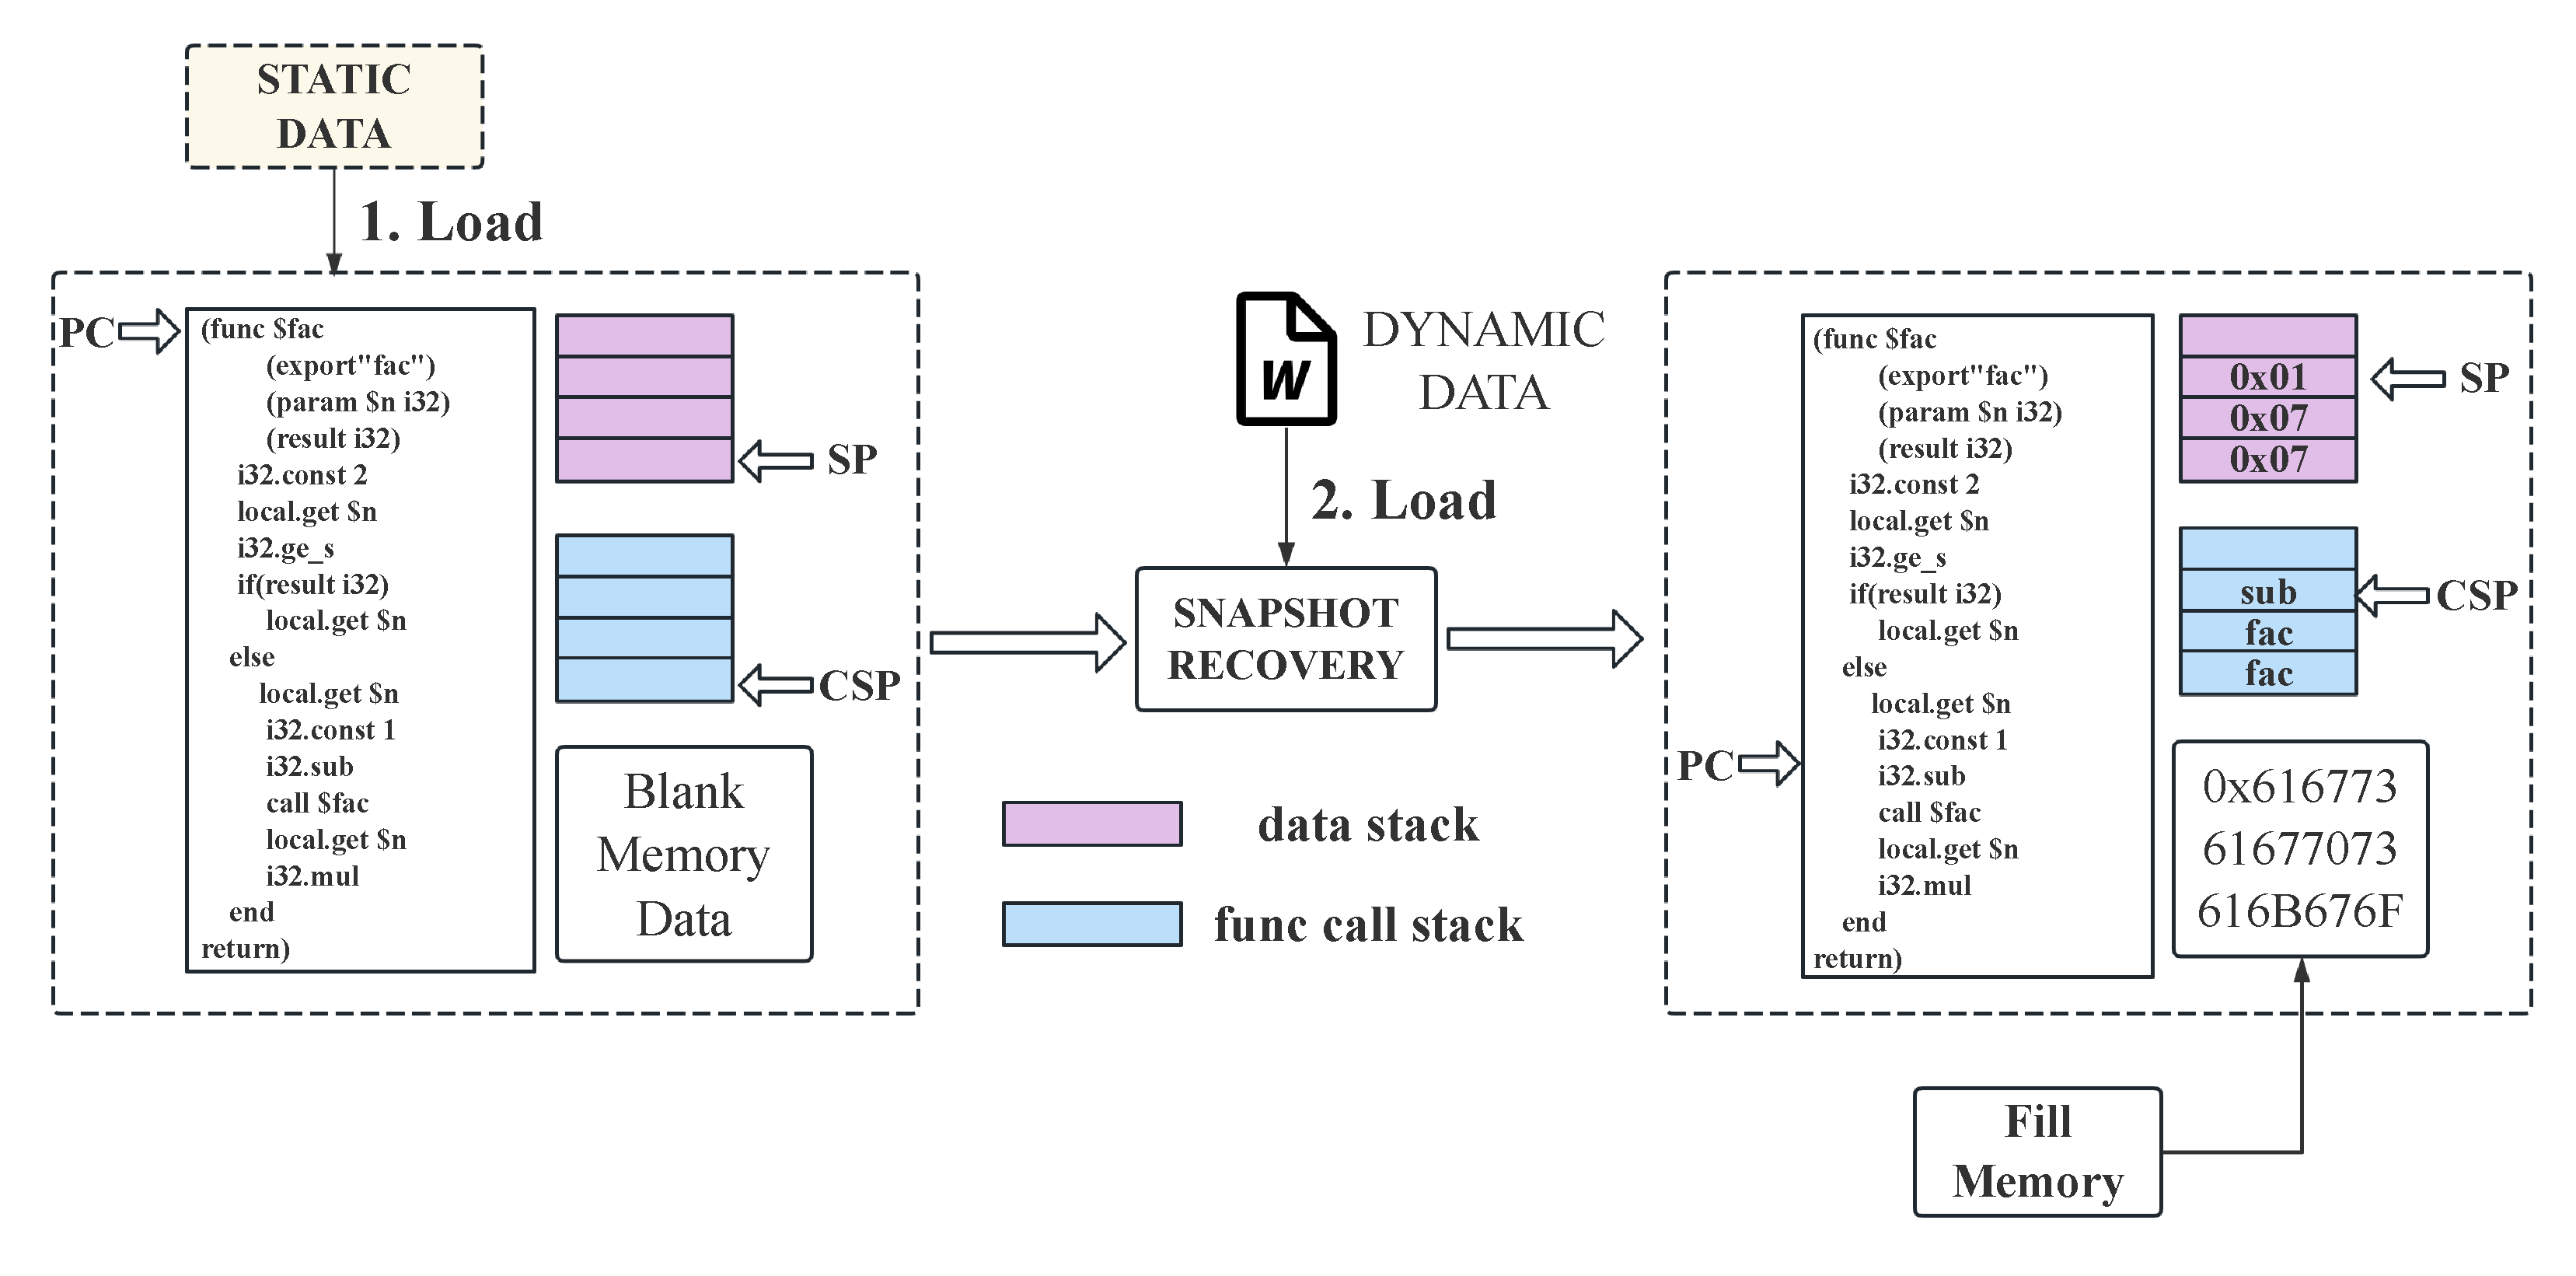
\includegraphics[width=0.75\linewidth]{BlkVc_load_image.pdf}
	\caption{Load Snapshot Details}
	\label{fig:blkvcloadimage}
\end{figure}


As shown in Figure~\ref{fig:blkvcloadimage}, when verifiers need to restore a specific runtime state from a snapshot file, they first load the static data. Since the static data remains unchanged throughout the execution of the entire computation task, only a single copy is required. Once the static data is loaded, the dynamic data is then applied to reconstruct the runtime state of the WASM-SNAP, restoring the state as it was when the snapshot was saved.


\subsubsection{Standardization for Snapshot Preservation}

After loading the compiled computation code, WASM-SNAP executes the instructions sequentially. CleVer assigns a specific weight to each instruction, which is equivalent to the execution time overhead of the instruction under the blockchain verification node environment. Furthermore, these instruction weights can be flexibly adjusted based on the hardware configurations of different blockchain verification nodes. To fully utilize the on-chain verification environment, CleVer sets the snapshot-saving instruction threshold to align with the standard block production time of the blockchain.

In Definition~\ref{def:snap-standard}, we define the instruction threshold standard $T_w$ for state preservation. During computation or verification, WASM-SNAP tracks the cumulative weight of the executed instructions. Once the cumulative weight exceeds the saving threshold, WASM-SNAP automatically saves a snapshot and resets the cumulative weight to zero, then continues with the computation. The same rule is applied during the verification process by verifiers and when arbitrating computational correctness on-chain.


\subsection{Incentive-Accumulated Challenge Verification}

During the challenge verification phase, verifiers who detect errors will directly initiate a single-step challenge, with the blockchain arbitrating whether the challenge is valid. Under normal protocol, erroneous computational snapshots will always be challenged on-chain.

However, if a malicious attacker continuously occupies the on-chain challenge interface—meaning they repeatedly submit challenges against correct snapshots—this could prevent honest verifiers' challenges from being processed on-chain. As a result, the erroneous task will be incorrectly recognized as correct within the system.

Based on this, we provide the following definition.

\begin{definition}
    During the challenge verification phase, challenges can be categorized into two types based on the nature of the challenger:
    \begin{itemize}
        \item \textbf{Honest Challenge.} \textnormal{ Initiated by an honest verifier. When the verifier detects an error in the task, it raises a challenge directly against the detected issue. }
        \item \textbf{Invalid Challenge.} \textnormal{ Initiated by a malicious adversary (i.e., a malicious verifier). The goal is to occupy the challenge window, thereby preventing honest challenges from taking place and causing the system to incorrectly accept an invalid task as correct. }
    \end{itemize}
\end{definition}

To solve this problem, CleVer proposes a verification scheme with cumulative incentives. Table~\ref{tab:payoff-fs} describes the incentive scheme for verifiers who submitted correct verification results in round~$s$.


\paragraph{General staking and reward pool}
Let $f:\mathbb{N}\to\mathbb{R}_{>0}$ be a \emph{strictly increasing} staking function; each round-$s$ participant escrows $f(s)$ and pays a per-round fee $\mathrm{fee}>0$. Let $B\ge0$ be a base bounty posted for the dispute. Denote by $N_i\in\mathbb{N}$ the number of invalid challengers penalized in round $i$. The cumulative \emph{reward pool} before deciding round $s$ is
\[
\mathrm{Pool}(s)\;=\;B+\sum_{i=1}^{s-1} N_i\,f(i)
\]
If an honest challenge is admitted at round $s$, the winner(s) obtain $\mathrm{Pool}(s)$ (pro rata) and their deposit $f(s)$ is returned; fees are never refunded. An invalid challenger forfeits its deposit into future pools.

\begin{remark}[Round index and Sybil-robustness]
The round counter $s$ is per-dispute and increases with each adjudicated round \emph{independent of identity}, preventing an adversary from "resetting" $s$ via Sybil identities.
\end{remark}

\begin{table}[h]
\centering
\caption{Payoff summary under a general staking schedule $f(s)$}
\renewcommand{\arraystretch}{1.2}
\begin{tabular}{lcc}
\toprule
Event & Deposit at round $s$ & Net payoff at round $s$ \\
\midrule
Honest Challenge & $f(s)$ (returned) & $\mathrm{Pool}(s)-\mathrm{fee}$ \\
Invalid Challenge & $f(s)$ (forfeited) & $-\big(f(s)+\mathrm{fee}\big)$ \\
\bottomrule
\end{tabular}
\label{tab:payoff-fs}
\vspace{-0.6em}
\end{table}

\paragraph{Notation}
Let $F(t)=\sum_{i=1}^{t} f(i)$ be the cumulative staking function and define the (integer) generalized inverse
\[
F^{-1}(y)\;=\;\max\{\,t\in\mathbb{N}:\,F(t)\le y\,\}\quad(y\ge 0)
\]

\begin{theorem}[Generic finality bound]\label{thm:generic-finality}
Assume $f$ is strictly increasing. Suppose at least one invalid challenge is submitted in each of the first $t$ rounds (worst case for liveness). The coalition’s cumulative loss satisfies
\[
L(t)\;\ge\;\sum_{i=1}^{t}\big(f(i)+\mathrm{fee}\big)\;=\;F(t)+t\,\mathrm{fee}
\]
Consequently, with adversarial budget $C>0$, the maximal sustainable blocking rounds obey
\[
t(C)\;\le\;F^{-1}(C)\,,
\]
and an honest challenge must be admitted by round $s^\star\le t(C)+1$. Finality is thus reached within $F^{-1}(C)+1$ rounds (ignoring fees; fees only decrease $t(C)$).
\end{theorem}

\begin{proof}
Each invalid round costs at least $f(i)+\mathrm{fee}$. If the adversary blocks $t$ rounds, then $L(t)\ge F(t)+t\,\mathrm{fee}$. The constraint $L(t)\le C$ implies $F(t)\le C$, so $t\le F^{-1}(C)$, hence $s^\star\le t+1$.
\end{proof}

\begin{theorem}[Profitability threshold for honest challengers]\label{thm:profit-fs}
In the above worst case, the net payoff of a successful honest challenge at round $s$ satisfies
\[
\mathrm{profit}(s)\;\ge\;B+F(s-1)\;-\;\mathrm{fee}.
\]
Therefore:
\begin{enumerate}
  \item If $B\ge \mathrm{fee}$, every admitted honest challenge is non-negative from $s=1$ onward.
  \item In general, the smallest profitable round is
  \[
    s_{\min}\;=\;1+F^{-1}\!\big((\mathrm{fee}-B)_+\big), \quad (x)_+=\max\{x,0\}
  \]
\end{enumerate}
\end{theorem}

\begin{proof}
Since at least one invalid challenger is penalized in each blocked round, we have $\mathrm{Pool}(s)\ge B+F(s-1)$. Profit equals $\mathrm{Pool}(s)-\mathrm{fee}$. The claims follow by solving $B+F(s-1)\ge \mathrm{fee}$ for $s$.
\end{proof}

\begin{lemma}[Multi-attacker amplification]\label{lem:multi}
If in each blocked round there are at least $m\ge1$ invalid challengers (i.e., $N_i\ge m$ for all $i$ before admission), then
\[
\mathrm{Pool}(s)\;\ge\;B+m\,F(s-1)\quad\text{and}\quad
L(t)\;\ge\;m\,F(t)+t\,m\,\mathrm{fee}
\]
Hence, with adversarial coalition budget $C$, the sustainable blocking rounds satisfy
\[
t(C)\;\le\;F^{-1}\!\Big(\tfrac{C}{m}\Big)
\]
and the profitability threshold improves to
\[
s_{\min}\;=\;1+F^{-1}\!\big(\tfrac{(\mathrm{fee}-B)_+}{m}\big)
\]
\end{lemma}

\begin{proof}
Each blocked round penalizes at least $m$ deposits of size $f(i)$, so $\mathrm{Pool}(s)\ge B+\sum_{i=1}^{s-1} m f(i)=B+mF(s-1)$. The coalition’s per-round loss is at least $m(f(i)+\mathrm{fee})$, yielding $L(t)\ge mF(t)+tm\mathrm{fee}$. The bounds follow by repeating the arguments of Theorems~\ref{thm:generic-finality} and~\ref{thm:profit-fs} with the factor $m$.
\end{proof}

\begin{corollary}[Few-round finality under multiplicative growth]\label{cor:multiplicative}
If $f$ satisfies $f(s+1)\ge (1+\gamma)f(s)$ for some $\gamma>0$ (hence $f(s)\ge f(1)(1+\gamma)^{s-1}$), then for adversarial budget $C$:
\[
t(C)\;\le\;\left\lfloor \log_{1+\gamma}\!\Big(1+\tfrac{\gamma\,C}{f(1)}\Big)\right\rfloor
\;=\;\mathcal{O}\!\big(\log C\big)
\]
Under the multi-attacker condition of Lemma~\ref{lem:multi}, this sharpens to
\[
t(C)\;\le\;\left\lfloor \log_{1+\gamma}\!\Big(1+\tfrac{\gamma\,C}{m\,f(1)}\Big)\right\rfloor
\]
i.e., finality in a \emph{logarithmic} number of rounds, accelerated by the factor $m$.
\end{corollary}

\begin{proof}
Geometric lower bounds give $F(t)\ge f(1)\big((1+\gamma)^t-1\big)/\gamma$. Combine with Theorem~\ref{thm:generic-finality}; then apply Lemma~\ref{lem:multi} for the $m$-amplified case and solve for $t$.
\end{proof}

\begin{corollary}[Other growth regimes]\label{cor:other}
If $f(s)\ge a\,s^{k}$ with $k\ge 1$, then $F(t)\ge \frac{a}{k+1}t^{k+1}$ and
\[
t(C)\;\le\;\Big(\tfrac{(k+1)C}{a}\Big)^{\!\frac{1}{k+1}} \quad
\text{(polynomial growth $\Rightarrow$ sublinear rounds)}
\]
If $f(s)\ge a\log(s+1)$, then $F(t)\ge a\sum_{i=1}^{t}\log(i+1)\approx a\,(t\log t - t)$, so $t(C)$ grows superlinearly in $C$ (weakest deterrence). Under Lemma~\ref{lem:multi}, replace $C$ by $C/m$ to obtain the corresponding tightened bounds.
\end{corollary}

\section{Anonymous Verification of Computation} \label{sec:anony}

This section introduces the entire verification process of the anonymous verifier mechanism and explains the anonymous verifier election mechanism in detail. This mechanism is a key component in ensuring the security of the challenge verification system while protecting the anonymity of verifiers and preventing them from being targeted by malicious attacks.



\subsection{Generic Construction}

\subsubsection{Intuition}

CleVer's anonymous verification protocol ensures the privacy of verifier identities while effectively mitigating the verifier dilemma. Specifically, each user who registers as a verifier must perform anonymous staking, during which verifiable anonymous identity information is provided. Verifiers register in the system using a unique nullifier $N_i$, which ensures both confidentiality and unpredictability. During task verification, verifiers record intermediate snapshot weights as a proof of verification workload. When interacting with the blockchain, they must submit this proof together with a zk-membership proof of their anonymous identity.

After staking is completed, the system enters the verification phase, during which verifiers use zk-SNARKs to prove the correctness of their staking note. In particular, when generating anonymous staking data, the node includes a unique commitment $C_{\text{stake}}$ that conceals the real identity and serves as a staking credential for interacting with the system.

\begin{figure}[H]
    \centering
    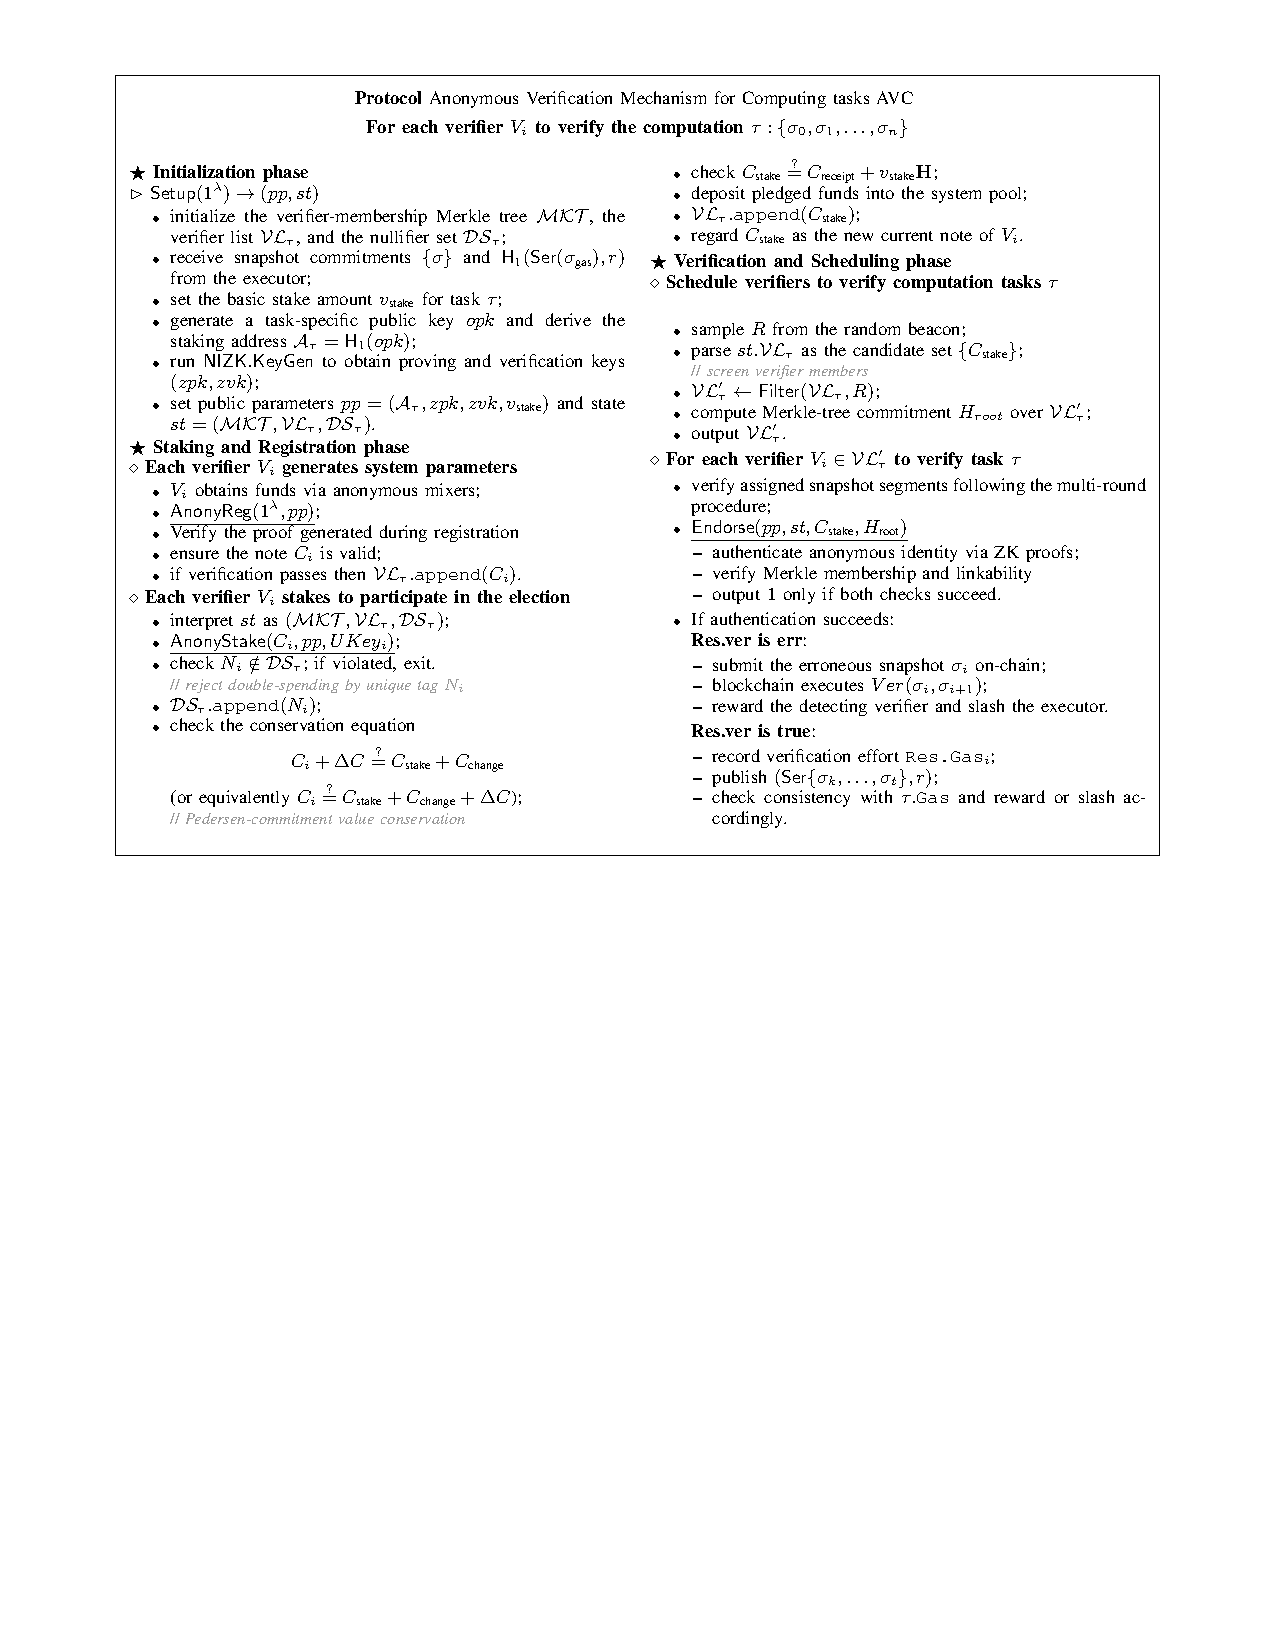
\includegraphics[width=1.0\linewidth]{AVC.pdf}
    \caption{Anonymous Verification Mechanism for Computing Tasks}
    \label{ASCE}
\end{figure}

To verify the correctness of the staked amount, we utilize Pedersen commitments to conceal the specific staking value. Leveraging its additive homomorphism, we construct a balancing term $\Delta C$ to verify value conservation. Additionally, we introduce a nullifier $N_i$ to prevent double-spending attacks, ensuring the uniqueness and security of each staking transaction.

The verifier identities remain unlinkable across different tasks because  each participation uses a fresh commitment and nullifier, preventing cross-task linkage.

\subsubsection{Construction}

\begin{figure}[htbp]
    \centering
    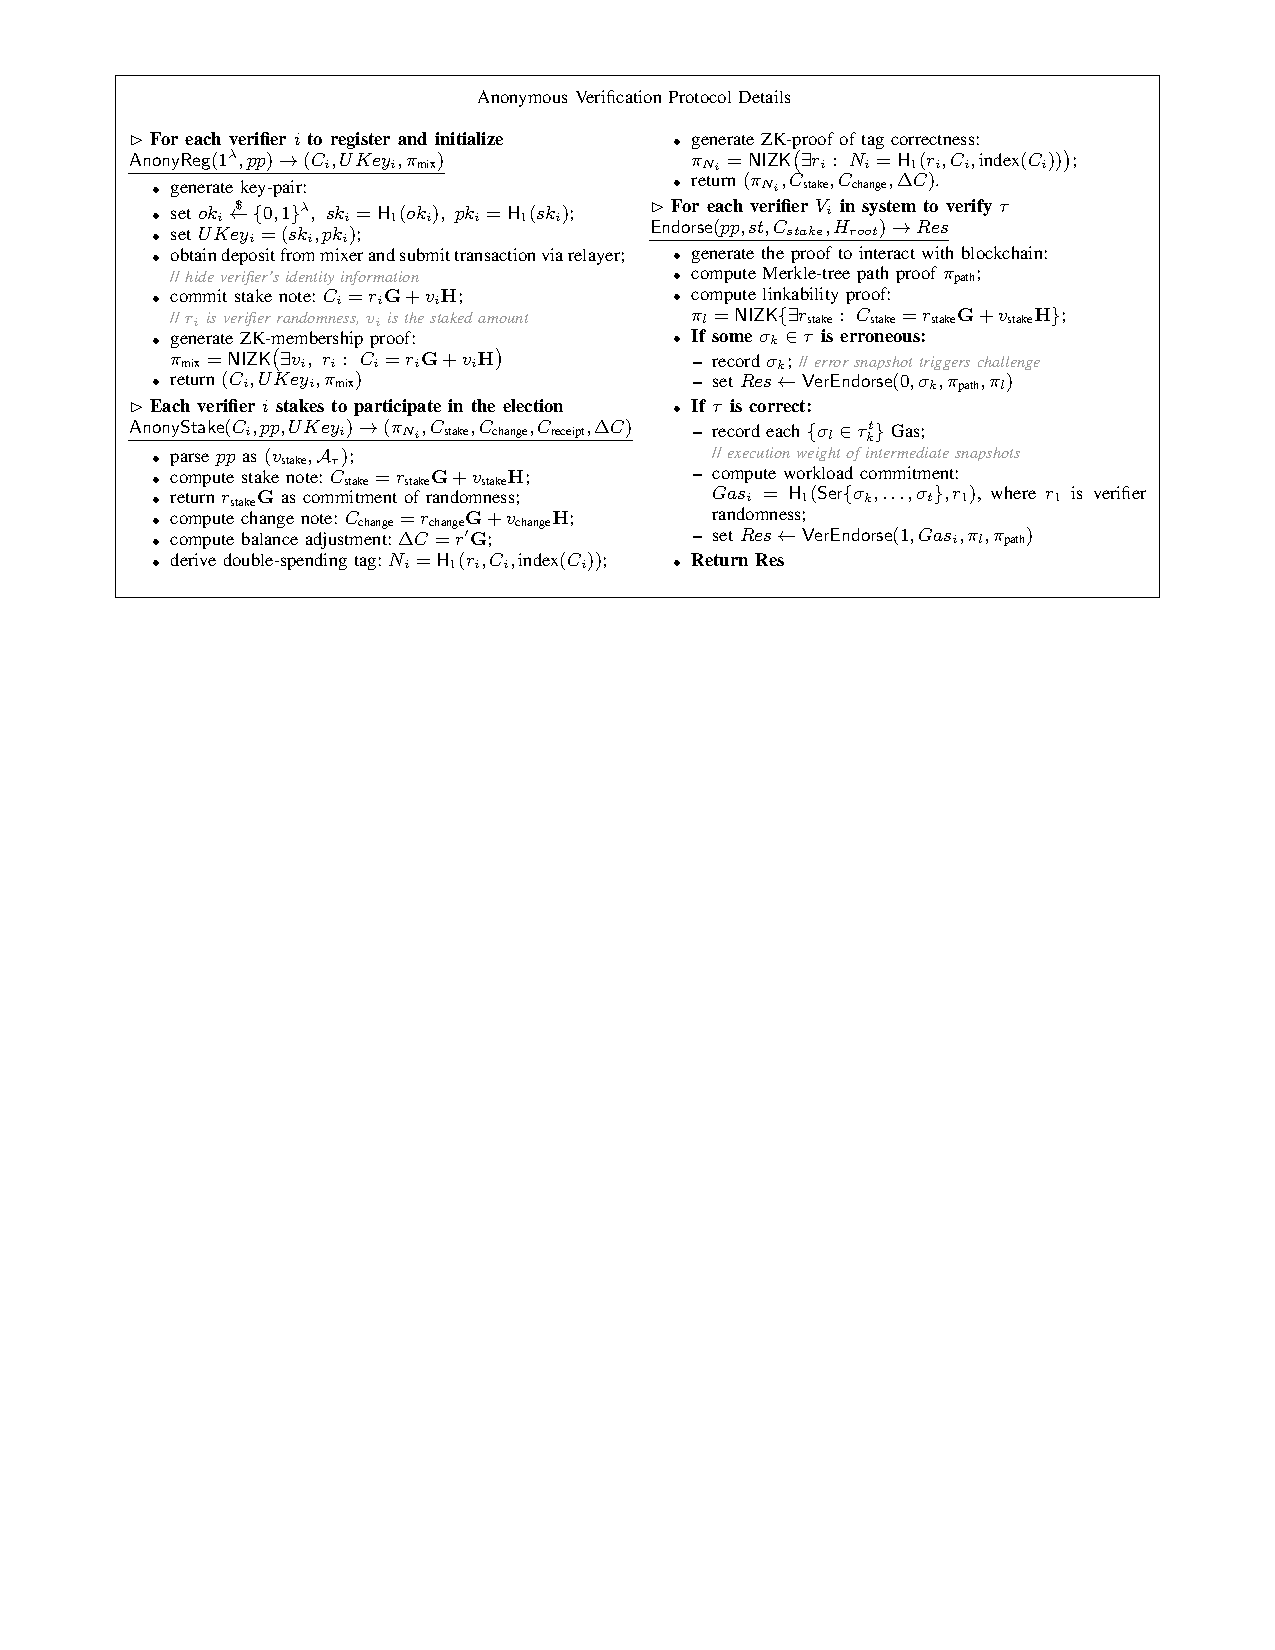
\includegraphics[width=1\linewidth]{AVPD.pdf}
    \caption{Anonymous Verification Protocol Details}
    \label{CVP}
\end{figure}

The protocol is described in Figure~\ref{CVP}, containing the following components:

\begin{itemize}
    \item \textbf{Initialization Phase:} The system first needs to be initialized, including the public data structures and the public parameters about $\tau$, and then the participating verifiers generate the associated keys.
    \item \textbf{Staking and Registration Phase:} Nodes that participate in anonymous staking can apply to join the verification system. During the anonymous staking process, an identity identifier is generated. Additionally, all successfully staked nodes will be compiled into a global list, which is used to select verifiers.
    \item \textbf{Verification Phase:} The system assigns a group of verifiers to each task. The verifiers then perform the task verification, and if an error is detected, they initiate a one-step challenge on the blockchain. Based on the final verification result, the blockchain enforces rewards and penalties for the parties involved.
\end{itemize}

\subsection{ Verifier-Side Protocol Details }

The protocol describes the overall process of anonymous verification of computing tasks. Next, we detail the key functions.

\[
\underline{ \mathsf{AnonyReg}(1^\lambda, pp) \rightarrow (C_i, UKey_i, \pi_{\text{mix}}) }
\]

In the anonymous registration phase, verifiers complete key generation, anonymous deposit, and system registration.

\begin{enumerate}[label=(\arabic*)]
    \item \textbf{Key Generation.}
    Each verifier generates a personal key pair and a random scalar $r_i$, which is used to construct a Pedersen commitment and also serves as part of the verifier’s anonymous identity.
    \item \textbf{Anonymous Registration.}
    To prevent Sybil attacks, the system requires verifiers to deposit a certain amount of funds before they can participate. Verifiers anonymously deposit funds via a mixer. During this process, the verifier generates a commitment $C_i$ together with a zk-membership proof $\pi_{\text{mix}}$ attesting to well-formedness/membership (without revealing the amount). Upon successful verification, $C_i$ is bound to verifier $V_i$ as their anonymous identifier.

\end{enumerate}

\[
\underline{ \mathsf{AnonyStake}(C_i, pp, UKey_i) \rightarrow (\pi_{N_i}, C_{\text{stake}}, C_{\text{change}}, C_{\text{receipt}}, \Delta C) }
\]

\begin{enumerate}[label=(\arabic*)]
    \item \textbf{Stake Preparation.}
    The prover selects the input note \( C_i \) (current balance/identity). According to the staking parameters, two output notes are computed: the staking note \( C_{\text{stake}} \) and the change note \( C_{\text{change}} \), ensuring value conservation and uniqueness.
    \item \textbf{Proof Generation.}
    Compute the nullifier \( N_i=\hash_1(r_i, C_i, \text{index}) \) to prevent double-spending, and generate a zk-proof \( \pi_{N_i} \) proving ownership of \( C_i \) and correctness of the outputs without revealing sensitive information.
    \item \textbf{Staking and Broadcasting.}
    The prover packages the transaction and broadcasts it. The transaction includes \( C_i \), \( C_{\text{stake}} \), \( C_{\text{change}} \), the receipt commitment \( C_{\text{receipt}} \), the nullifier \( N_i \), and \( \pi_{N_i} \).
    \item \textbf{Verification and State Update.}
    The system verifies the zk-proof and checks whether \( N_i \) has been used. If valid, the staking note is accepted as locked capital and the system state is updated.
\end{enumerate}

The verifier anonymously stakes assets by splitting an input note $C_i$ into a staking note $C_{\text{stake}}$ and a change note $C_{\text{change}}$. A nullifier $N_i$ and zk-proof are generated to ensure correctness and prevent double-spending without revealing private information.

\[
\underline{ \mathsf{Endorse}(pp, st, C_{\text{stake}}, H_{root}) \rightarrow Res }
\]

\begin{enumerate}[label=(\arabic*)]
    \item \textbf{Identity Proof Generation.}
    The verifier proves membership via a Merkle path proof $\pi_{\text{path}}$ under $H_{root}$, ensuring only authorized verifiers participate. Next, a linkability proof $\pi_l$ is generated to confirm that the staking note $C_{\text{stake}}$ is bound to the verifier’s anonymous registration, preventing impersonation while preserving anonymity.
    \item \textbf{Verification of Computation Tasks.}
    Upon receiving a computational task, the verifier examines the task’s set of slices. If any error is detected, the verifier initiates a one-step on-chain challenge and certifies the task as incorrect.
    \item \textbf{Endorsement of Task Correctness.}
    If the computation is correct, the verifier endorses it and records the workload commitment (the weights of intermediate snapshot transitions) to prevent the verifier dilemma.
\end{enumerate}

\subsection{Protocol Correctness Explanation}

\textbf{Anonymity Explanation.}
Each verifier creates an identity commitment $C$ using a Pedersen commitment as an anonymous tag. A relay hides the transaction source during blockchain interactions. When submitting verification results, the verifier uses a zk-SNARK to prove knowledge of the corresponding randomness $r_{\text{stake}}$, thereby achieving anonymous identity authentication. No real-world identity information is exposed.

\textbf{Staking Correctness Explanation.}
Verifiers participate by staking funds. By value conservation $v_i = v_{\text{stake}} + v_{\text{change}}$. A balancing term $\Delta C$ preserves randomness. The system checks
\[
C_i + \Delta C = C_{\text{stake}} + C_{\text{change}}
\]
i.e.,
\[
(r_i + r')G + v_iH = (r_{\text{stake}} + r_{\text{change}})G + (v_{\text{stake}} + v_{\text{change}})H
\]
where $r'$ is the randomness of $\Delta C$. To prevent double-spending, each verifier must submit a nullifier $N_i$ bound to $(r_i,C_i)$; the system ensures $N_i$ is not reused.


\section{Security Analysis}

The core purpose of CleVer is to ensure that off-chain computation tasks can be efficiently verified on-chain. In this section, we analyze the system’s anonymity properties, demonstrating that verifiers can participate in the protocol without exposing their identities to potential external attacks.Building on this, we further analyze the security of the verification functionality, showing that the system can maintain its intended verification behavior even under various attack scenarios. Additionally, incentive compatibility is fundamental to the correct operation of the system. We prove that CleVer’s incentive mechanism satisfies incentive compatibility, ensuring that all parties are motivated to behave as intended.

\subsection{System Anonymity Analysis}

In CleVer, verifiers complete identity registration through anonymous staking. Each verifier generates their anonymous identity based on a Pedersen commitment. Due to the computational hiding and binding properties of Pedersen commitments, an adversary cannot infer the underlying randomness from the public commitment $C_i$.

To prevent on-chain identity linkage, all funds are anonymously injected into the system via a mixer, effectively breaking the traceability between the fund source and the verifier's identity. Furthermore, all blockchain interactions are broadcast through a relayer, which hides the true sender address of transactions and protects against identity inference attacks based on network-level or on-chain transaction analysis. When submitting validation results, verifiers generate a zero-knowledge proof using a combination of zk-SNARKs and Merkle proofs, proving their membership in the verifier set without revealing any specific identity within the set.

To prevent adversaries from forging identities in system, CleVer requires each verifier to submit a zero-knowledge ownership proof during protocol interactions, proving knowledge of the randomness $r_i$ corresponding to their identity commitment $C_i$. This proof is constructed using zk-SNARKs and is bound to a unique nullifier $N_i$ to prevent double-spending and replay attacks.

\subsection{Honest Verification in the System}

In CleVer, verifiers incur costs when participating in the system and performing verification tasks. Due to the existence of a punishment mechanism and the high likelihood of tasks being correctly executed, some verifiers may choose to skip actual verification and simply endorse the correctness of computation results to save costs. On the other hand, some may attempt to free-ride by following the actions of other verifiers without performing the verification themselves. CleVer mitigates this “Verifier Dilemma” through a cumulative weight recording mechanism.

\begin{theorem}[Succinct Proof of Verifier Effort]
CleVer employs an execution-weight-based tracking and verification mechanism that enables verifiers to provide succinct proofs of their verification effort. This mechanism satisfies the following properties:

\begin{itemize}
  \item \textbf{Correctness}: Verifiers who honestly execute the computation task can generate a proof of effort that passes verification;
  \item \textbf{Unforgeability}: Verifiers who do not perform the actual computation cannot forge a valid proof of effort except with negligible probability;
  \item \textbf{Succinctness}: The cost of verifying a submitted proof is significantly lower than re-executing the computation task.
\end{itemize}

Therefore, this mechanism effectively avoids the verifier dilemma and incentivizes verifiers to perform verification honestly.
\end{theorem}

\begin{proof}
By definition, the computation task $\tau$ is represented by a program $P$ loaded into our customized WASM-SNAP execution environment. Given an initial state $\sigma_{\text{start}}$, the execution of $P$ follows a deterministic instruction trace $(i_1, i_2, \ldots, i_m)$, where each instruction $i_j$ has an associated fixed weight $w(i_j) \in \mathbb{N}$.

The system defines a cumulative weight threshold $T_w$. During the execution of $\tau$, the verifier maintains a counter that records the cumulative weight. Whenever the accumulated weight is about to exceed $T_w$, the segment is recorded and the counter is reset. Let the recorded weight segments throughout execution form the sequence:

\[
W = (w_1, w_2, \ldots, w_n), \quad \text{where} \quad \sum_{j=1}^{n} w_j = \sum_{j=1}^{m} w(i_j)
\]

The honest prover computes a reference sequence $W_{\text{ref}}$ during execution, which serves as the verification standard.

\textbf{1. Correctness:}  
CleVer executes computation tasks in the deterministic WASM-SNAP environment. The program $P$ has a unique execution trace $I$ under input $x$, and each instruction has a fixed weight. Therefore, the sequence $W$ generated by an honest verifier will match the reference sequence $W_{\text{ref}}$ exactly.

\textbf{2. Unforgeability:}  
Without re-execution from the committed snapshots, producing a matching sequence and digest chain would require breaking the hash function’s collision resistance; therefore the success probability is negligible.


\textbf{3. Succinctness:}  
The verifier only needs to compare the submitted sequence $W$ with the reference $W_{\text{ref}}$, which requires $O(n)$ time. Since $n \ll m$, this is far more efficient than re-executing the full program, whose complexity is $O(m)$. Thus, verification is significantly cheaper.

\textbf{4. Avoiding the Verifier Dilemma:}  
Since verifiers are required to submit verifiable proofs of verification, and invalid or missing proofs lead to penalties—while forgery is nearly impossible—the rational strategy for verifiers is to perform honest verification. This effectively resolves the verifier dilemma.

In summary, the execution-weight-based tracking and verification mechanism in CleVer satisfies correctness, unforgeability, and succinct verification. It provides a practical and secure approach for enforcing honest verifier behavior in a public blockchain setting.
\end{proof}

\subsection{Incentive Compatibility of the System}

CleVer ensures that the system operates correctly according to the protocol by achieving incentive compatibility under honest strategies for all participating roles.

\begin{definition}[Stubborn Verifier Adversary]
A stubborn verifier adversary is one who, upon entering a challenge window, persistently occupies the window by submitting invalid challenges until its budget is depleted.
\end{definition}

In CleVer, provided that there exists at least one honest verifier for each task, the correctness of an incorrect computation can be guaranteed once an honest challenge is admitted. By Theorem~\ref{thm:generic-finality}, an adversary with bounded budget can block only finitely many rounds. In particular, under multiplicative growth of the staking function $f(s)$ (Corollary~\ref{cor:multiplicative}), the number of blocking rounds grows only logarithmically in the adversary’s budget, ensuring rapid termination. Meanwhile, as the reward pool accumulates with each blocked round (Theorem~\ref{thm:profit-fs} and Lemma~\ref{lem:multi}), rational stakeholders are incentivized to fund honest verifiers, making timely challenges economically attractive.

\begin{theorem}
Suppose the dispute allows at most $k$ challenge rounds. If the following conditions hold, the system outputs a correct verification conclusion:
\begin{itemize}
    \item The adversary’s budget is bounded by $C$ with
    \[
    C \;<\; \sum_{i=1}^{k}\big(f(i)+\mathrm{fee}\big)
    \]
    i.e., the adversary cannot afford to block all $k$ rounds;
    \item The cumulative reward/penalty mechanism yields positive expected payoff for an admitted honest challenge (cf.\ Theorem~\ref{thm:profit-fs} and Lemma~\ref{lem:multi}), so that a rational stakeholder will fund an honest verifier to submit a challenge.
\end{itemize}
\end{theorem}

\begin{proof}
By Theorem~\ref{thm:generic-finality}, blocking the first $k$ rounds requires a cumulative expenditure of at least $\sum_{i=1}^{k}\big(f(i)+\mathrm{fee}\big)$. If $C$ is smaller than this amount, the adversary can block at most $k-1$ rounds, and an honest challenge is admitted by round $k$ (or earlier). Under multiplicative growth of $f(s)$ (Corollary~\ref{cor:multiplicative}), the number of blocking rounds is only logarithmic in $C$, guaranteeing rapid termination and a correct verification outcome.
\end{proof}

Based on the above analysis, CleVer makes honest behavior strictly more profitable than dishonest behavior. The utilities of different roles are summarized as follows:

\begin{itemize}
\item \textbf{Honest verifier (task correct):} When the task is correct, the verifier receives the protocol-defined attestation reward (strictly positive by design in the system model).

\item \textbf{Honest challenger (task incorrect):} When the task is incorrect, an honest verifier (possibly funded by stakeholders) initiates a challenge. By Theorem~\ref{thm:profit-fs}, cumulative incentives guarantee a non-negative (and beyond the threshold, strictly positive) return once admitted.

\item \textbf{Stakeholders:} Rational stakeholders can fund honest challengers to share cumulative rewards; their utility is proportional to investment, ensuring incentive alignment (see Lemma~\ref{lem:multi} for accelerated accumulation under multiple invalid challengers).

\item \textbf{Bribery attack:} Verifier anonymity makes targeted bribery infeasible in practice, substantially weakening bribery-based deviations.

\item \textbf{Abuse of the challenge interface:} By Theorem~\ref{thm:generic-finality}, repeated invalid challenges lead to strictly negative expected returns for adversaries, while honest challenges eventually prevail.

\item \textbf{Lazy verification strategy:} CleVer mitigates the \textbf{Verifier Dilemma} via succinct workload proofs; without performing actual verification, a verifier’s stake is slashed, rendering free-riding unprofitable.

\item \textbf{Malicious executor:} As specified in the system model, the executor’s base stake is parameterized to cover the potential reward pool of honest verifiers, ensuring economic soundness.
\end{itemize}

\noindent In summary, for rational verifiers and stakeholders, honest verification and timely challenges yield stable and strictly positive returns, whereas malicious strategies produce negative or zero payoff. Therefore, CleVer satisfies incentive compatibility under honest strategies.


\section{Experiment and comparison}

In this section, we evaluate CleVer from both a theoretical and an empirical perspective. The experiments are organized into three parts. First, we perform a structural comparison against existing blockchain-based verification frameworks, focusing on their verification assumptions, redundancy overhead, and asymptotic finality behaviors. Since prior schemes such as Truebit, Arbitrum, and state channel–based designs are typically analyzed through their asymptotic verification models rather than implementation-level metrics, we present this comparison in a theoretical manner consistent with how these schemes are evaluated in the literature. This allows us to highlight CleVer’s core advantage—reducing unnecessary dispute rounds and avoiding redundant recomputation—which is most naturally measured at the analytical level (Table~\ref{tab:scheme-compare} and Figure~\ref{fig:finality-fs}). 

Next, we evaluate CleVer’s verification performance on actual workloads using our WASM-SNAP execution environment. These experiments measure concrete factors such as verification delay, storage overhead, and incentive cost trade-offs across different verification modes, as well as CleVer’s scalability on large and computation-intensive tasks. Finally, we benchmark the cryptographic components used in the anonymous verifier protocol to assess practicality in real-world deployment. Together, these complementary evaluations—analytical comparison for structural properties and empirical benchmarks for realized performance—provide a complete assessment of CleVer’s verification capabilities.

\subsection{Compare to Blockchain Verification Project}

We compare CleVer with existing blockchain projects that support the verification of complex computations. The comparison primarily focuses on three aspects: their underlying security assumptions, the redundancy of execution, and whether they support general-purpose computation (i.e., whether the verification mechanism is computation-agnostic).

Furthermore, we evaluate and compare their verification performance, including the finality rounds, as well as the verification cost.

\begin{table}[htbp]
\centering
\caption{Comparison with blockchain verification schemes\tnote{1}}
\label{tab:scheme-compare}
\setlength{\tabcolsep}{4pt}
\renewcommand{\arraystretch}{1.15}
\footnotesize
\begin{threeparttable}
\begin{tabular}{
    p{2.0cm}
    >{\centering\arraybackslash}p{1.8cm}
    >{\centering\arraybackslash}p{2.1cm}
    >{\centering\arraybackslash}p{1.5cm}
    >{\centering\arraybackslash}p{3.0cm}
    >{\centering\arraybackslash}p{3.0cm}
}
\toprule
\textbf{Protocol} & \textbf{Assumption} & \textbf{Redundancy} & \textbf{Agnosticism} &
\textbf{Finality rounds\tnote{2}} & \textbf{Verification cost} \\
\midrule
Split~\cite{luu}            & BAR & $O(n)$                 & \ding{51} & $O(W_\tau)$                                 & $n a_{\tau}$ \\
Probability~\cite{luu}      & BAR & $O(n)$                 & \ding{55} & $O(1)$                                      & $n a_{\tau}$ \\
State Channel~\cite{GenSTATE}    & BA  & $O(1)\mid O(n)$        & \ding{55} & $O(1)\mid \infty$                           & $0 \mid \log n \cdot a_{\tau}$ \\
Arbitrum~\cite{ARBITRUM1}         & BR  & $O(1)\mid O(n)$        & \ding{55} & $O(1)\mid O(B_\mathcal{A}\log W_\tau)$      & $0 \mid \tfrac{1}{P_g} a_{\tau} + W_\tau\, \mathit{fee}$ \\
Truebit~\cite{TRUEBIT}          & BR  & $O(1)\mid O(n)$        & \ding{51} & $O(1)\mid \infty$                           & $a_{\tau} \mid a_{\tau} + \log(P_g)\,\mathit{fee}$ \\
\textbf{CleVer(Our Scheme)}  & BR  & $O(1)\mid O(m)$        & \ding{51} & $O(1)\mid O(F^{-1}(B_\mathcal{A}))$         & $a_{\tau} + \mathit{fee}$ \\
\bottomrule
\end{tabular}

\begin{tablenotes}\footnotesize
\item[1] See Table~\ref{Notations} for the definitions and units of
$W_\tau$, $a_\tau$, $B_\mathcal{A}$ and $\mathit{fee}$.
\item[2] Finality rounds denote the number of verification rounds from task submission
to termination. For CleVer:
\begin{itemize}
    \item Exponential $f(s)$ ($f(s+1)\ge (1+\gamma)f(s)$): $O(\log B_\mathcal{A})$ rounds.
    \item Linear $f(s)=a s$: $O(\sqrt{B_\mathcal{A}})$ rounds.
    \item Logarithmic $f(s)=a\log(s+1)$: superlinear in $B_\mathcal{A}$ (weakest deterrence).
\end{itemize}
\item[3] $B$, $A$, and $R$ denote Byzantine (arbitrary adversarial), Altruistic (always follow protocol),
and Rational (utility-maximizing) nodes, respectively.
\end{tablenotes}
\end{threeparttable}
\end{table}


\begin{figure}[htbp]
    \centering
    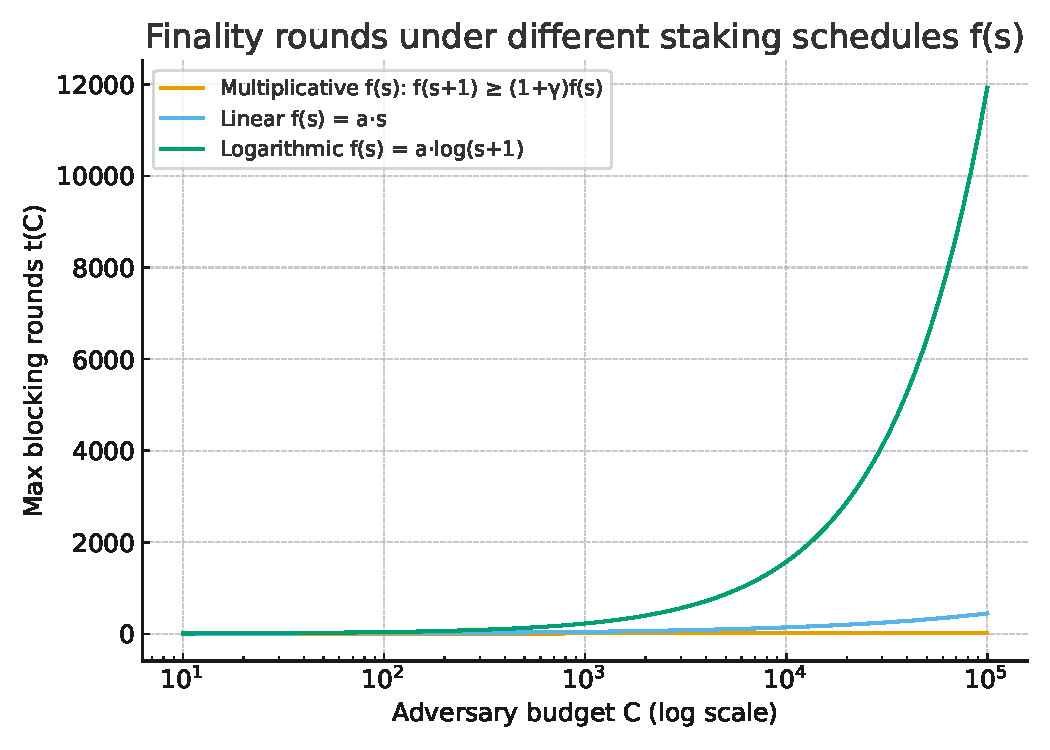
\includegraphics[width=0.6\linewidth]{finality_rounds.pdf}
    \caption{Finality rounds $t(C)$ under different staking schedules $f(s)$. 
    Multiplicative growth ensures logarithmic termination, linear growth yields sublinear rounds, 
    while logarithmic growth results in weaker deterrence.}
    \label{fig:finality-fs}
\end{figure}

We use $O(1)\mid \mathrm{Inf}$ to represent the optimistic and worst cases respectively. From the analysis of the table, we can see that the two solutions proposed by Luu et al.~\cite{luu}, the former directly splits the task into multiple subtasks for verification on-chain but brings unbearable rounds of judgment and overhead, while the latter can only be applied to tasks with perfect decomposition. The state channel can only support complex transactions optimistically; once a dispute occurs, finality is lost. Arbitrum and Truebit both rely on binary decomposition, but Arbitrum’s challenge interface can be abused by stubborn adversaries, and Truebit is vulnerable to Sybil attacks once the identity-splitting incentive falls below verification cost.

In contrast, \textbf{CleVer} adopts a cumulative staking-based optimistic verification model. In its general form, the finality round complexity is $O(F^{-1}(B_\mathcal{A}))$, where $F$ is the cumulative staking function. Under exponential growth of $f(s)$, finality is logarithmic in the adversary’s budget, ensuring rapid termination. With linear growth, finality is sublinear, and with logarithmic growth, deterrence is weakest. This unified framework shows that CleVer flexibly balances security, efficiency, and accessibility depending on the choice of $f(s)$.


\subsection{General Purpose Computation Verification}

\begin{table}[htbp]
\centering
\caption{Task Performance Comparison}
\label{tab:general}
\footnotesize
\setlength{\tabcolsep}{3pt}  
\renewcommand{\arraystretch}{1.2}
\begin{tabular}{
    >{\centering\arraybackslash}p{0.18\linewidth}  % Task
    >{\centering\arraybackslash}p{0.14\linewidth}  % Input Size
    >{\centering\arraybackslash}p{0.12\linewidth}  % Native Time
    >{\centering\arraybackslash}p{0.12\linewidth}  % Snap Time
    >{\centering\arraybackslash}p{0.11\linewidth}  % Static Size
    >{\centering\arraybackslash}p{0.15\linewidth}  % Dynamic Size
    >{\centering\arraybackslash}p{0.10\linewidth}  % Ver Cost
}
\toprule
\textbf{Computation Task} &
\textbf{Input Size} &
\textbf{Native Time(s)} &
\textbf{Snap Time(s)} &
\textbf{Static Size(Bytes)} &
\textbf{Dynamic Size(MB)} &
\textbf{$Ver(\cdot)$ Cost(s)} \\
\midrule
Heap Sort &
$2{\cdot}10^5,\;5{\cdot}10^5,\;10^6$ &
2.43 / 6.51 / 13.70 &
2.94 / 8.59 / 18.77 &
89 &
0.78 / 1.02 / 1.08 &
2.46 \\
Fibonacci sequence &
35 &
3.85 &
4.73 &
859 &
- &
0.65 \\
Fra.\ Image Gen &
$800{\times}800$ dpi &
12.22 &
15.13 &
312 &
0.04 &
2.13 \\
FNN (1 epoch) &
MNIST $28{\times}28$ &
46.72 &
68.67 &
493 &
0.39 &
9.95 \\
\bottomrule
\end{tabular}
\end{table}

CleVer is implemented based on the WebAssembly execution framework, supports general-purpose computing, and is highly adaptable. We evaluated the system's performance under both lightweight tasks (small snapshots) and complex workloads. Table~\ref{tab:general} shows that CleVer achieves efficient verification in these different scenarios. The weight of instructions in the snapshot is evaluated according to the block production time interval of the blockchain nodes, and the execution time of instructions in WASM-SNAP will not exceed the node block production time.

Table~\ref{vermodel} compares three verification modes. In the \textit{Follow} mode, the executor records frequent snapshots, increasing the number of verification rounds but reducing per-round latency and verifier incentives. In the \textit{Parallel} mode, multiple snapshots are retained and verified concurrently, significantly reducing verification delay at the cost of increased storage overhead. The \textit{Serial} mode records only state digests, requiring verifiers to perform sequential validation, which doubles delay but avoids large storage.

To further test scalability, we applied CleVer to compute the principal eigenvector of a $10^5 \times 10^5$ sparse matrix using power iteration within a single WASM-SNAP instance. The experiment ran for approximately 3000 seconds with several thousand iterations, and snapshots averaged around 260MB. CleVer maintained stable verification performance under these heavy workloads. Parallel mode achieved the lowest latency, while Follow mode reduced verifier cost but required more rounds. These results demonstrate CleVer’s ability to flexibly balance delay, storage, and incentive expenses, ensuring efficient verification for general-purpose computations.


\begin{table}[h]
\centering
\caption{CleVer's different verification modes$^1$}\label{vermodel}
\begin{tabular}{ccccc}
\toprule
\textbf{Verification Mode} & \textbf{Delay Cost} & \textbf{Storage Cost} & \textbf{Incentive Expenses} & \textbf{Rounds} \\
\midrule
Follow & $(1+ \frac{1}{10})A$ & - & $\frac{\mathcal{I}}{10}$ & $10k$ \\
Parallel & $(1+\frac{1}{32})A$ & 8.52Gb & $\mathcal{I}$ & $k$ \\
Serial & $2A$ & - & $\mathcal{I}$ & $k$ \\
\bottomrule
\end{tabular}

\begin{threeparttable}
\begin{tablenotes}
\footnotesize
\item[1] The computing party only record the summary of the intermediate state $\sigma_i$. If an error is detected during verification, the verifier will submit a complete snapshot for challenge. $A$ is baseline execution cost, and $\mathcal{I}$ is base incentive unit.
\end{tablenotes}
\end{threeparttable}

\vspace{-0.5em}
\end{table}


\subsection{Component Performance Test}

We used an Intel i5-12400H with 32GB RAM as the client environment to benchmark circuit compilation, trusted setup, and proof generation times for three zero-knowledge circuits ($\pi_{\text{mix}}, \pi_{N_i}, \pi_\ell$) using Circom and snarkJS. All proofs were generated in a single-threaded setting. To emulate a realistic production environment, on-chain verification performance was measured on a simulated blockchain node with an AMD EPYC 7302P and 64GB RAM.

\begin{table}[h]
\centering
\caption{Zero-knowledge proof microbenchmarks (Groth16, BN254)}
\label{tab:zkbench}
\begin{tabular}{lcccc}
\toprule
\textbf{Circuit} & \textbf{Compile Time} & \textbf{Proof Gen Time} & \textbf{Setup Time} \\
\midrule
$\pi_{\text{mix}}$ & 297\,ms & 2.4\,ms  & 1.2\,s \\
$\pi_{N_i}$        & 1.43\,s & 1.3\,s   & 5.2\,s \\
$\pi_\ell$         & 286\,ms & 2.3\,ms  & 1.1\,s \\
\bottomrule
\end{tabular}
\begin{minipage}{0.95\linewidth}\footnotesize
\textit{Notes.} Benchmarked on Intel i5-12400H (32GB RAM), single-threaded. 
Compile = circuit compilation; Setup = trusted parameter generation; Proof Gen = client-side proof generation using snarkJS. 
On-chain verification costs are reported separately in Figure~\ref{fig:gascost}.
\end{minipage}
\vspace{-0.5em}
\end{table}

The experimental results are shown in Table~\ref{tab:zkbench}. The proof generation time of $\pi_{N_i}$ is 1.3\,s, while the generation times of the other two proofs are within 300\,ms. The overhead remains within an acceptable range and demonstrates practical feasibility.

\begin{figure}[htbp]
	\centering
	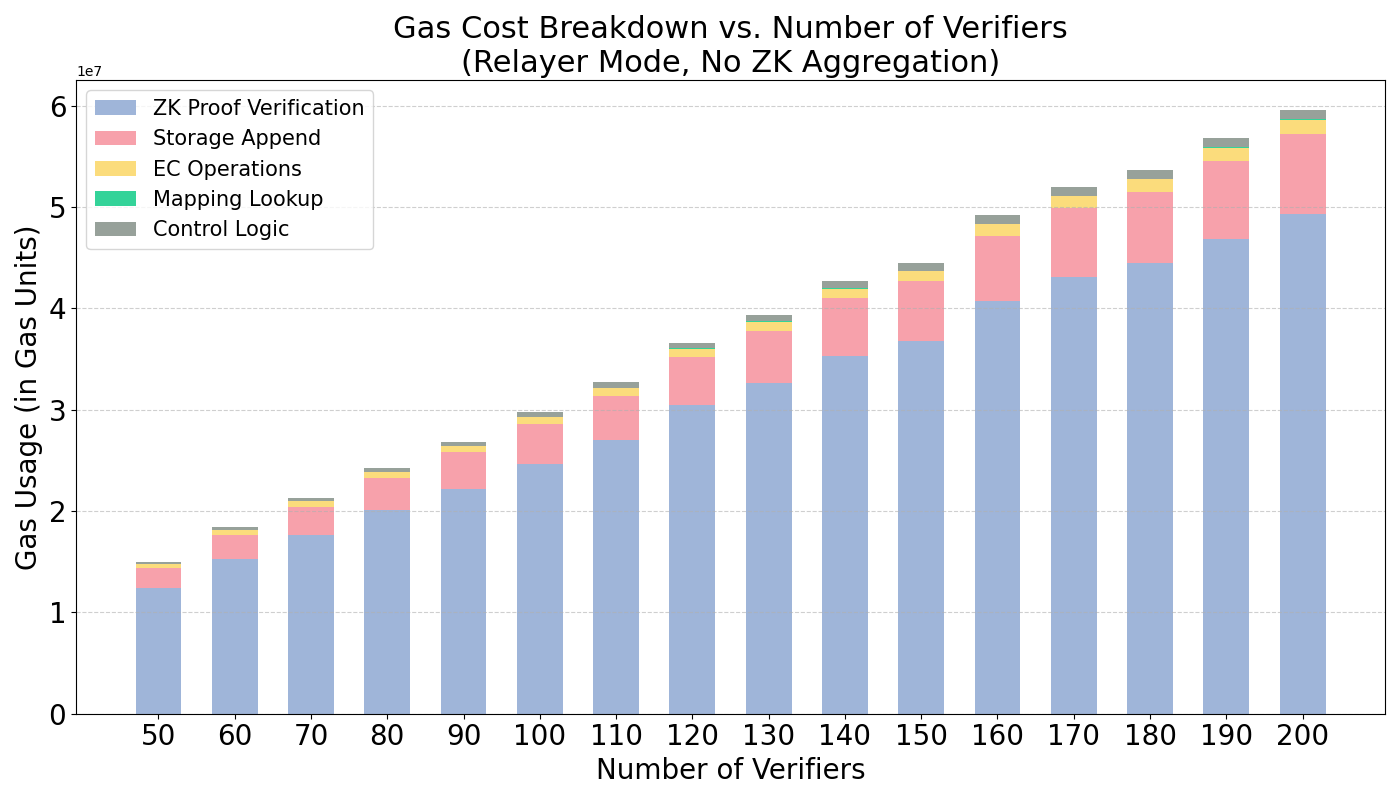
\includegraphics[width=0.7\linewidth]{GasCost.png}
	\caption{CleVer gas cost on-chain (EVM relayer mode, no ZK aggregation)}
	\label{fig:gascost}
\end{figure}

We also evaluated CleVer’s on-chain resource consumption on the EVM. Figure~\ref{fig:gascost} shows the breakdown of gas costs during batch operations performed by the relayer, without zero-knowledge aggregation, as the number of verifiers increases from 50 to 200. Gas usage grows approximately linearly with the number of verifiers. Based on typical gas prices, CleVer incurs very low per-execution costs—about \$0.005 on BSC and \$0.0024 on Polygon—demonstrating strong economic efficiency and scalability.


\section{Conclusion}

We propose CleVer, a novel verification framework that supports efficient and scalable verification of general-purpose computations. CleVer introduces a compute-and-leave model based on state snapshots, enabling off-chain execution without requiring expensive proof generation or circuit transformation. Through a single-step on-chain challenge protocol and an anonymous verifier election mechanism, CleVer ensures low-cost verification, strong security against bribery and DDoS attacks, and rapid finality. Our results demonstrate that CleVer achieves high performance, incentive compatibility, and broad applicability across complex computation scenarios.

\textbf{Limitations and future work.} CleVer still depends on the liveness and stability of the underlying blockchain, and prolonged congestion may delay challenge admission. In addition, verifiers must execute the full task, which may place higher hardware requirements on nodes for computation-intensive workloads. Future work will explore reducing verifier execution cost and designing adaptive, resource-aware verification strategies.

\section*{Acknowledgements}
This paper is supported by the National Key R\&D Program of China through project 2022YFB2702900, the Natural Science Foundation of China through projects U21A20467, U24B20144 and 62272464.

\section*{Declaration of Generative AI and AI-assisted Technologies in the Writing Process}

During the preparation of this work, the authors used \textit{ChatGPT (OpenAI)} for language polishing and logical consistency checking. After using this tool, the authors reviewed and edited the content as needed and take full responsibility for the content of this publication.


\bibliographystyle{elsarticle-num}
\bibliography{linkable}



\appendix

\end{document}
